\chapter{Diode Circuit I}

\section{Objectives}
\begin{itemize}
    \item To learn the basic property of a pn diode and a zener diode
    \item To construct simple circuits and verify their performance
\end{itemize}

\section{Materials}
\begin{itemize}
    \item Breadboard
    \item DC power supply
    \item Digital Multi-Meter
    \item \hyperref[1N4148]{Diode (1N4148)}
    \item Resistors
    \item \hyperref[SR160]{Schottky didode (SR160)}
    \item \hyperref[1N4728A]{Zener diode (1N4728A)}
\end{itemize}

\section{Introduction}
In this experiment, we are going to learn the features and properties of different diodes in the simple diode circuits. A DC source, resistors, PN diodes, a Zener diode, and a Schottky didode will be used to construct the circuits, the digital multi-meter is used to measure $V_x$ and $V_s$ to find the relationship between them.\par
    \subsection{Diodes}
    \FloatBarrier
        \begin{itemize}
            \item \textbf{What are the diodes}\par
                A diode is a two-terminal electronic component. It is normally made of silicon or other semiconducting materials such as gallium arsenide and germanium. It allows current to flow in one-direction with condition while blocking it in the opposite direction.\par
                Yet there is a situation that it can be broken down by applying a certain value of reverse voltage, which makes it damaged and becomes a permanent conductor irreversibly, this is called avalanche breakdown.$^{\ref{diode_vi}}$ Nevertheless, some of diodes are designed to accept reverse voltage, such as Zener diodes and Schottky diodes.$^{\ref{z_diode_vi}}$ The breakdown happens on these two diodes are reversible. \par
                \begin{figure}[h]
                    \centering
                    \begin{subfigure}[h]{0.45\textwidth}
                        \centering
                        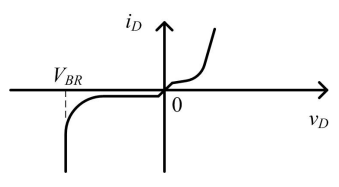
\includegraphics[width=0.9\linewidth]{Lab01/Lab1_diode_vi.png}
                        \caption{V-I Graph of Regular diodes}
                        \label{diode_vi}
                    \end{subfigure}
                    \hfill
                    \begin{subfigure}[h]{0.45\textwidth}
                        \centering
                        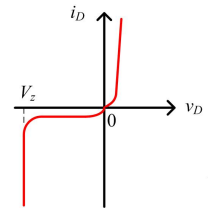
\includegraphics[width=0.6\linewidth]{Lab01/Lab1_zener_diode_vi.png}
                        \caption{V-I Graph of Zener diodes}
                        \label{z_diode_vi}
                    \end{subfigure}
                \end{figure}
                \FloatBarrier
                Diodes are widely used in electronic devices for tasks like rectification, circuit protection, and signal modulation.
                
            \item \textbf{Zener Diodes}\par
                Zener diode is the special type of diode, which is designed to allow current to flow in reverse direction when certain value of reverse voltage ($V_z$) is applied.
                
            \item \textbf{Schottky Diodes}\par
                Schottky diode is another specialized type of diode, it has a low forward voltage drop and a very fast switching action. Differ from diodes mentioned above, it is formed by the junction of a semiconductor with a metal.
        \end{itemize}
    \subsection{Specification}
        \begin{itemize}
            \item \hyperref[1N4148]{\textbf{Diode (1N4148)}}
            \item \hyperref[SR160]{\textbf{Schottky didode (SR160)}}
            \item \hyperref[1N4728A]{\textbf{Zener diode (1N4728A)}}
        \end{itemize}
    
\newpage
    \subsection{Circuit Diagram}
    \begin{figure}[h]

        \begin{subfigure}[h]{0.47\textwidth}
        \begin{center}
            \includesvg[width=1\linewidth]{Lab01/Lab1a.drawio.svg}
            \caption{}
            \label{Lab1a}
        \end{center} 
        \end{subfigure}
    \hfill
    \vspace{0.2 cm}
        \begin{subfigure}[h]{0.47\textwidth}
        \begin{center}
            \includesvg[width=1\linewidth]{Lab01/Lab1b.drawio.svg}
            \caption{}
            \label{Lab1b}
        \end{center}
        \end{subfigure}
    \vfill
    \vspace{0.2 cm}
        \begin{subfigure}[h]{0.47\textwidth}
        \begin{center}
            \includesvg[width=1\linewidth]{Lab01/Lab1c.drawio.svg} 
            \caption{}
            \label{Lab1c}
        \end{center}
        \end{subfigure}
    \hfill
        \begin{subfigure}[h]{0.47\textwidth}
        \begin{center}
            \includesvg[width=1\linewidth]{Lab01/Lab1d.drawio.svg}
            \caption{}
            \label{Lab1d}
        \end{center}
        \end{subfigure}
    \caption{Simlpe Diode Circuits}
    \label{SDC}

    \end{figure}
\FloatBarrier
The R shown in the circuits represents 1k$\Omega$. D is the unlabelled diode.


\section{Detailed Procedures}
    \subsection{Analyzation}
    First, we analyze the relationship between $V_s$ and $V_x$ in the circuits.\par
    The relationship between $V_i$ and $V_o$ is:\par
    \begin{itemize}
        \item In figure. \ref{Lab1a}:\par
        \begin{equation}
            \begin{cases}
                V_x = \frac{2}{3}V_s - V_\gamma & V_s \ge V_\gamma,~\text{D is on}\\
                V_x = 0 & V_s < V_\gamma,~\text{D is off}\\
            \end{cases}
        \label{l1eq1}
        \end{equation}
        
        \item In figure. \ref{Lab1b}:
        \begin{equation}
            \begin{cases}
                V_x = \frac{V_s+2V_\gamma}{3} & V_s\ge \frac{8}{5}V_\gamma,~\text{D is on}\\
                V_x = \frac{3V_s}{4} & V_s < \frac{8}{5}V_\gamma,~\text{D is off}\\
            \end{cases}
        \label{l1eq2}
        \end{equation}
            
        \item In figure. \ref{Lab1c}:
        \begin{equation}
            \begin{cases}
                V_x = \frac{5V_s+2V_\gamma}{7} & V_s > 8V_\gamma,~\text{$D_1$ is off \& $D_2$ is on}\\
                V_x = \frac{3V_s}{4} & -\frac{8}{5}V_\gamma \le V_s \le 8V_\gamma,~\text{Both diodes off}\\
                V_x = \frac{V_s-2V_\gamma}{3} & V_s < -\frac{8}{5}V_\gamma,~\text{$D_1$ is on \& $D_2$ is off}\\
            \end{cases}
        \label{l1eq3}
        \end{equation}
            
        \item In figure. \ref{Lab1d}:
        \begin{equation}
            \begin{cases}
                V_x = \frac{3V_s+V_Z}{4} & V_s > \frac{5}{3}V_Z,~\text{Diode is reverse conducting}\\
                V_x = \frac{9V_s}{10} & -\frac{5}{3}V_\gamma \le V_s \le \frac{5}{3}V_Z,~\text{Diode is not conducting}\\
                V_x = \frac{3V_s-V_\gamma}{4} & V_s < -\frac{5}{3}V_\gamma,~\text{Diode is forward conducting}\\
            \end{cases}
        \label{l1eq4}
        \end{equation}
    \end{itemize}
    \FloatBarrier
    Then we measure the data of each diode by using digital multi-meter:\par
    \begin{itemize}
        \item In Equation.\ref{l1eq1} and Equation.\ref{l1eq2},\par
        $V_\gamma$ = 0.5519V
        \item In Equation.\ref{l1eq3},\par
        $V_\gamma$ of $D_1$ = 0.5519V \& $V_\gamma$ of $D_2$ = 0.5440V 
        \item In Equation.\ref{l1eq4},\par
        $V_Z$ = -2.269V \& $V_\gamma$ = 0.666V
        \item For Schottky Diode,\par
        $V_\gamma$ = 0.1653V
    \end{itemize}
    \FloatBarrier
    
    
    \subsection{Procedures}
    We used digital multi-meter to measure $V_x$ when $V_s$ varies:\par
    \begin{itemize}
        \item For Fig.\ref{Lab1a},\par
            \begin{table}[h]
            \centering
            \begin{tabular}{|c|c|c|c|c|c|c|c|c|}
            \hline
                $V_s$ & -1     & -0.8  & -0.6  & -0.4  & -0.2  & 0     & 0.2   & 0.4   \\ \hline
                $V_x$ & 0      & 0     & 0     & 0     & 0     & 0     & 0.25m & 7.3m  \\ \hline
                Theo  & 0      & 0     & 0     & 0     & 0     & 0     & 0     & 0     \\ \hline
                $V_s$ & 0.6    & 0.8   & 1     & 1.2   & 1.4   & 1.6   & 1.8   & 2     \\ \hline
                $V_x$ & 47.2m  & 99.5m & 0.158 & 0.219 & 0.280 & 0.344 & 0.407 & 0.473 \\ \hline
                Theo  & 0.0173 & 0.084 & 0.151 & 0.217 & 0.284 & 0.351 & 0.417 & 0.484 \\ \hline
            \end{tabular}
            \end{table}
            \FloatBarrier
        \item For Fig.\ref{Lab1b},\par
            \begin{table}[h]
            \centering
            \begin{tabular}{|c|c|c|c|c|c|c|c|c|}
            \hline
                $V_s$ & -1     & -0.8   & -0.6   & -0.4   & -0.2  & 0      & 0.2   & 0.4   \\ \hline
                $V_x$ & -0.752 & -0.601 & -0.447 & -0.299 & -0.15 & -0.006 & 0.150 & 0.298 \\ \hline
                Theo  & -0.75  & -0.6   & -0.45  & -0.3   & -0.15 & 0      & 0.15  & 0.3   \\ \hline
                $V_s$ & 0.6    & 0.8    & 1      & 1.2    & 1.4   & 1.6    & 1.8   & 2     \\ \hline
                $V_x$ & 0.439  & 0.560  & 0.652  & 0.736  & 0.817 & 0.892  & 0.963 & 1.036 \\ \hline
                Theo  & 0.45   & 0.6    & 0.699  & 0.765  & 0.832 & 0.899  & 0.965 & 1.032 \\ \hline
            \end{tabular}
            \end{table}
            \FloatBarrier
        \item For Fig.\ref{Lab1c},\par
            \begin{table}[h]
            \centering
            \resizebox{\columnwidth}{!}{
            \begin{tabular}{|c|c|c|c|c|c|c|c|c|c|c|c|c|}
            \hline
                $V_s$ & -4     & -3.5   & -3     & -2.5   & -2     & -1.5   & -1     & -0.5   & 0      & 0.5   & 1     & 1.5   \\ \hline
                $V_x$ & -1.739 & -1.566 & -1.394 & -1.217 & -1.039 & -0.854 & -0.656 & -0.372 & -0.006 & 0.374 & 0.752 & 1.124 \\ \hline
                Theo  & -1.733 & -1.563 & -1.389 & -1.216 & -1.035 & -0.850 & -0.652 & -0.370 & 0      & 0.372 & 0.748 & 1.120 \\ \hline
                $V_s$ & 2      & 2.5    & 3      & 3.5    & 4      & 4.5    & 5      & 5.5    & 6      & 6.5   & 7     &       \\ \hline
                $V_x$ & 1.503  & 1.877  & 2.252  & 2.622  & 2.994  & 3.363  & 3.724  & 4.089  & 4.45   & 4.812 & 5.173 &       \\ \hline
                Theo  & 1.497  & 1.878  & 2.247  & 2.620  & 2.984  & 3.361  & 3.720  & 4.084  & 4.440  & 4.804 & 5.169 &       \\ \hline
            \end{tabular}
            }
            \end{table}
            \FloatBarrier
        \item For Fig.\ref{Lab1d},\par
            \begin{table}[h]
            \centering
            \resizebox{\columnwidth}{!}{
            \begin{tabular}{|c|c|c|c|c|c|c|c|c|c|c|c|c|}
            \hline
                $V_s$ & -4      & -3.5    & -3      & -2.5    & -2      & -1.5    & -1      & -0.5    & 0       & 0.5     & 1       & 1.5  \\ \hline
                $V_x$ & -3.191  & -2.817  & -2.44   & -2.062  & -1.687  & -1.304  & -0.950  & -0.449  & 0.01    & 0.445   & 0.897   & 1.34 \\ \hline
                Theo  & -3.1665 & -2.7915 & -2.4165 & -2.0415 & -1.6665 & -1.2915 & -0.9    & -0.45   & 0       & 0.45    & 0.9     & 1.35 \\ \hline
                $V_s$ & 2       & 2.5     & 3       & 3.5     & 4       & 4.5     & 5       & 5.5     & 6       & 6.5     & 7       &      \\ \hline
                $V_x$ & 1.793   & 2.23    & 2.688   & 3.134   & 3.575   & 4.014   & 4.444   & 4.861   & 5.272   & 5.681   & 6.081   &      \\ \hline
                Theo  & 1.8     & 2.25    & 2.7     & 3.15    & 3.56725 & 3.94225 & 4.31725 & 4.69225 & 5.06725 & 5.44225 & 5.81725 &      \\ \hline
            \end{tabular}
            }
            \end{table}
            \FloatBarrier
    \end{itemize}
    

\section{Discussion}
    In reality case, the resistance of resistor and the build-in voltage of diode are not ideal, and this leads to the difference between theoretical value and measured value. In this experiment, we measured all the resistors used in the circuit, the mean errors of the resistors is 2.78\%, the build-in voltage values of diode we took are $V_\gamma$ = 0.7, or $V_\gamma$ = 0.666 and $V_Z$ = -2.269 in different cases.\par
    Furthermore, in calculation, we always take the diode ideally, which it turns to a zero resistance component when it is on. The actual diodes do not change immediately from non-conducting to no-impedance when the voltage across it exceeds threshold voltage (As Fig.\ref{diode_vi} shown).\par
    Overall, the practical condition is always not the same as ideal condition, so it will result in differences in outcomes.

\section{Conclusion}
    In conclusion, we conduct serials of experiment and built four different circuits with different diodes. And this experiment has provided me a deeper understanding about the diodes.\par
    The standard diode shows the fundamental property of allowing current to flow only the way when the potential difference across it is positive. However, even if the potential difference is positive, the diode does not allow current to pass unless the voltage exceeds the threshold value. Else If the potential difference is negative, the diode blocks current flow.\par
    On the other hand, the Zener diode presents a unique characteristic which is it allows two-way conduction under specific conditions. When the reverse voltage exceeds the Zener breakdown voltage, the diode begins to conduct in the reverse direction. Or when the forward voltage exceeds the threshold voltage, it begins forward conduction.\par
    Overall, the experiments strengthened the knowledge of diode characteristics, including their threshold voltage and behavior under different biasing conditions.